\section{Control via backstepping}\label{sec:backstepping}
In this section we will present the backstepping control technique applied to the helicopter model. The main idea is to act on the whole system to ultimately obtain global asymptotic stability and therefore track a desired trajectory.
Let us consider once again the state-space representation in \ref{eq:fbl_model}. In order to find an analytical solution to the control problem, we will assume that the horizontal components of the control input $u$ (defined in \ref{eq:u}) are negligible. This is justified by the fact that, in nominal operational conditions, the main contribution of the thrust generated by the rotors is the vertical one with respect to the body frame. Therefore $u$ can be written as: 
\begin{align}
    u=
    \begin{bmatrix} 
        0 \\ 0 \\ u_3
    \end{bmatrix}. \label{eq:u3}
\end{align}

The objective is to design a control law $(u, \tau_{tot}^b)$, depending only on the measurable states, such that the tracking error
\begin{align*}
    \varepsilon(t) \coloneq (P(t)-P^d(t),W_3(t)-W_3^d(t))
\end{align*}
is asymptotically stable for all initial conditions.

We start the procedure with the definition of the position error in the body reference frame:
\begin{align*}
    \delta_1 \coloneq R^T(P^d-P).
\end{align*}
Its time derivative is given by:
\begin{align*}
    \frac{d}{dt}\delta_1 &= -\Omega^b \times R^T(P^d-P) + R^T \left( \frac{d}{dt}P^d-\frac{d}{dt}P \right) \\
    &= -\Omega^b \times \delta_1+R^T \left( \frac{d}{dt}P^d-V^b \right).
\end{align*}
From this, we identify the velocity error in the body reference frame:
\begin{align*}
    \delta_2 \coloneq R^T \left( \frac{d}{dt}P^d-V^b \right).
\end{align*}
After differentiation with respect to time, we obtain:
\begin{align*}
    \frac{d}{dt}\delta_2 &= -\Omega^b \times \delta_2+R^T \frac{d^2}{dt^2}P^d-\frac{1}{m}(R^T F_g^i -u).
\end{align*}

Define as $V_1$ the first Lyapunov function, regarding the pseudo-energy of the position and velocity errors, as:
\begin{align*}
    V_1 \coloneq \frac{1}{2}(\delta_1+\lambda \delta_2)^T(\delta_1+\lambda \delta_2)+\frac{1}{2}\delta_1^T\delta_1,
\end{align*}
where $\lambda>0$ is a slack variable to be tuned. The time derivative of $V_1$ is:
\begin{align*}
    \frac{d}{dt}V_1 = (\delta_1+\lambda \delta_2)^T \left( \delta_2+\lambda R^T \frac{d^2}{dt^2}P^d-\frac{\lambda}{m}u \right)+\delta_1^T \delta_2.
\end{align*} \\
We are looking for a virtual control input $(\frac{\lambda}{m}u)^*$ making $\frac{d}{dt}V_1 \leq -V_1$ barring an error that has to be recovered in the next iteration of the backstepping procedure. The aforementioned virtual control is:
\begin{align*}
    \left( \frac{\lambda}{m}u \right)^* = \delta_1+\lambda \delta_2+2\delta_2+\lambda R^T \frac{d^2}{dt^2}P^d.
\end{align*}
This choice results in:
\begin{gather*}
    \frac{d}{dt}V_1 = -(\delta_1+\lambda \delta_2)^T(\delta_1+\lambda \delta_2)-\lambda \delta_2^T \delta_2 + \\
    (\delta_1+\lambda \delta_2)^T \delta_3,
\end{gather*}
where:
\begin{align*}
    \delta_3 \coloneq \left( \frac{\lambda}{m}u \right)^*-\frac{\lambda}{m}u.
\end{align*}

We proceed further by computing the time derivative of $\delta_3$ as:
\begin{gather*}
    \frac{d}{dt}\delta_3 = -\Omega^b \times \delta_3 -\frac{\lambda}{m}\Omega^b \times u+\frac{\lambda+2}{\lambda}\delta_3-\frac{\lambda+2}{\lambda}\delta_1 \\
    -\frac{(\lambda+2)^2-\lambda}{\lambda}\delta_2+\lambda R^T \frac{d^3}{dt^3}P^d-\frac{\lambda}{m}\frac{d}{dt}u.
\end{gather*}
Let us consider at this stage the error in the yaw component:
\begin{align*}
    \varepsilon_2 = W_3^d-W_3.
\end{align*}
The second Lyapunov function is:
\begin{align*}
    V_2 = \frac{1}{2}\delta_3^T\delta_3+\frac{1}{2}\varepsilon_2^2,
\end{align*}
with its time derivative being:
\begin{gather*}
    \frac{d}{dt}V_2 = \delta_3^T \bigg( -\Omega^b \times \delta_3-\frac{\lambda}{m}\Omega^b \times u - \frac{\lambda+2}{\lambda}\delta_1 + \\
    \frac{\lambda+2}{\lambda}\delta_3 - \frac{(\lambda +2)^2 - \lambda}{\lambda} \delta_2 + \lambda R^T \frac{d^3}{dt^3}P^d - \frac{\lambda}{m} \frac{d}{dt} u \bigg) \\
    + \varepsilon_2 \left( \frac{d}{dt}{W_3^d}-\frac{d}{dt}W_3 \right).
\end{gather*}

The third component\footnote{Notice that $\delta_3^T  (-\Omega^b \times \delta_3) = 0$ and $\Omega^b \times u = \begin{bmatrix}
    \star & \star & 0
\end{bmatrix}^T.$} of the first bracket in the previous equation can be directly shaped by imposing the value of the derivative of the lift $u$:
\begin{gather*}
    \frac{d}{dt}u_3 =  \frac{m}{\lambda} \begin{bmatrix}
        0 & 0 & 1 \end{bmatrix} \bigg( \frac{\lambda+2}{\lambda}\delta_3-\frac{\lambda+2}{\lambda}\delta_1 \\ -\frac{\lambda^2+3\lambda+4}{\lambda}\delta_2+\lambda R^T \frac{d^3}{dt^3}P^d+ \delta_1+\lambda \delta_2 \bigg).
\end{gather*}
The vector $\begin{bmatrix}
    0 & 0 & 1
\end{bmatrix}$ has been used to isolate the third component of the equation. The residual positional error is taken into account with the goal of imposing the decrease rate of $\frac{d}{dt} (V_1 + V_2)$ along the system trajectories with the choice of the virtual control:
\begin{gather*}
    \left( \frac{\lambda}{m} \Omega^b \times u \right)^* \coloneq \begin{bmatrix}
        1 & 0 & 0 \\ 0 & 1 & 0 \\ 0 & 0 & 0
    \end{bmatrix} \bigg( \frac{\lambda+2}{\lambda}\delta_3-\frac{\lambda+2}{\lambda}\delta_1 \\ -\frac{\lambda^2+3\lambda+4}{\lambda}\delta_2+\lambda R^T \frac{d^3}{dt^3}P^d+ \delta_1+\lambda \delta_2 + k_1 \delta_3 \bigg).
\end{gather*}
that lives in the orthogonal plane to $u_3$, where $k_1>0$ is slack variable to be tuned in order to determine the rate of convergence of the error $\delta_3$.\\
Through the last two choices, we have only controlled the part of $\frac{d}{dt}V_2$ regarding the position error.
Now we can focus on the yaw term by introducing the virtual control:
\begin{gather*}
    \left( \frac{d}{dt}W_3 \right)^* \coloneq \frac{d}{dt}W_3^d + k_2 \varepsilon_2,
\end{gather*}
The derivative of the second Lyapunov function becomes:
\begin{gather*}
    \frac{d}{dt}V_2 = \delta_3^T \delta_4-k_1 \delta_3^T \delta_3 - \delta_3^T (\delta_1+\lambda \delta_2)  - k_2 \varepsilon_2^2 + \varepsilon_2 \varepsilon_3,
\end{gather*}
where:
\begin{gather*}
    \delta_4 \coloneq \left( \frac{\lambda}{m} \Omega^b \times u \right)^* - \frac{\lambda}{m} \Omega^b \times u, \\
    \varepsilon_3 \coloneq \frac{d}{dt}W_3^* - \frac{d}{dt}W_3.
\end{gather*}

Finally, the last iteration starts with the computation of the time derivative of the latter:
\begin{gather*}
    \frac{d}{dt}\delta_4 = \frac{d}{dt} \left( \frac{\lambda}{m} \Omega^b \times u \right)^* - \frac{\lambda}{m} \left( \frac{d}{dt} \Omega^b \right) \times u  \\ - \frac{\lambda}{m} \Omega^b \times \left( \frac{d}{dt} u \right), \\
    \frac{d}{dt} \varepsilon_3 = \frac{d^2}{dt^2} W_3^d + k_2 \bigg(\frac{d}{dt} W_3^d - \frac{d}{dt} W_3 \bigg) - \frac{d^2}{dt^2} W_3.
\end{gather*}
At this point, we can define the third Lyapunov function and proceed as usual.
\begin{gather*}
    V_3 = \frac{1}{2} \delta_4^T \delta_4 + \frac{1}{2} \varepsilon_3^2.
\end{gather*}
Which, after differentiation, results in:
\begin{gather*}
    \frac{d}{dt}V_3 = \delta_4^T \bigg( \frac{d}{dt} \left( \frac{\lambda}{m} \Omega^b \times u \right)^* - \frac{\lambda}{m} \left( \frac{d}{dt} \Omega^b \right) \times u \\ - \frac{\lambda}{m} \Omega^b \times \left( \frac{d}{dt} u \right) \bigg) \\
    + \varepsilon_3 \bigg( \frac{d^2}{dt^2} W_3^d + k_2 \bigg( \frac{d}{dt} W_3^d - \frac{d}{dt} W_3 \bigg) - \frac{d^2}{dt^2} W_3 \bigg).
\end{gather*}
Once again, our  goal is to "stabilize" the function $\frac{d}{dt}V_3$. This can be achieved through the following choices:
\begin{align*}
	\frac{d^2}{dt^2} W_3 = \frac{d^2}{dt^2} W_3^d + k_2\bigg( \frac{d}{dt} W_3^d - \frac{d}{dt} W_3 \bigg) + k_4\varepsilon_3 + \varepsilon_2,
\end{align*}
\begin{gather*}
	 \frac{\lambda}{m} \left( \frac{d}{dt} \Omega^b \right) \times u =  \frac{d}{dt} \left( \frac{\lambda}{m} \Omega^b \times u \right)^* - \frac{\lambda}{m} \Omega^b \times \left(\frac{d}{dt} u\right) \\ + \begin{bmatrix} 1 & 0 & 0 \\ 0 & 1 & 0 \\ 0 & 0 & 0 \end{bmatrix}\delta_3 + k_3\delta_4.
\end{gather*}
The very last equation results into the following expressions for the derivatives of the angular velocities in the body frame:
\begin{gather*}
	\frac{d}{dt} \Omega^b_1 = -\frac{m}{\lambda u_3}\begin{bmatrix}0 & 1 & 0\end{bmatrix}\bigg[ \frac{d}{dt} \left( \frac{\lambda}{m} \Omega^b \times u \right)^* -\\ \frac{\lambda}{m} \Omega^b \times \left(\frac{d}{dt} u\right) + \delta_3 + k_3\delta_4 \bigg], \\
	\frac{d}{dt} \Omega^b_2 = \frac{m}{\lambda u_3}\begin{bmatrix}1 & 0 & 0\end{bmatrix}\bigg[ \frac{d}{dt} \left( \frac{\lambda}{m} \Omega^b \times u \right)^* -\\ \frac{\lambda}{m} \Omega^b \times \left(\frac{d}{dt} u\right) + \delta_3 + k_3\delta_4 \bigg].
\end{gather*}
According to the above choices, the derivative of the third Lyapunov function becomes:
\begin{align*}
	\frac{d}{dt}V_3 = -k_4\varepsilon^2_3 - \varepsilon_2\varepsilon_3 - \delta_4^T\delta_3 - k_3\delta_4^T\delta_4.
\end{align*}

To summarize, consider the sum of the three aforementioned Lyapunov functions as the overall Lyapunov function $V$:
\begin{gather*}
	V=V_1+V_2+V_3=\frac{1}{2}(\delta_1+\lambda\delta_2)^T(\delta_1+\lambda\delta_2)+\\\frac{1}{2}\delta_1^T\delta_1+\frac{1}{2}\delta_3^T\delta_3+\frac{1}{2}\epsilon_2^2+\frac{1}{2}\delta_4^T\delta_4+\frac{1}{2}\epsilon_3^2,
\end{gather*}
with its time derivative being:
\begin{gather*}
	\frac{d}{dt}V=-(\delta_1+\lambda\delta_2)^T(\delta_1+\lambda\delta_2)-\lambda\delta_2^T\delta_2-k_1\delta_3^T\delta_3\\-k_2\varepsilon_2^2-k_4\varepsilon_3^2-k_3\delta_4^T\delta_4,
\end{gather*}
meaning that $V$ is monotonically decreasing (and thus the control objective is achieved) if and only if we pick the following:
\begin{gather*}
    \frac{d}{dt}u_3 =  \frac{m}{\lambda} \begin{bmatrix}
        0 & 0 & 1 \end{bmatrix} \bigg( \frac{\lambda+2}{\lambda}\delta_3-\frac{\lambda+2}{\lambda}\delta_1 \\ -\frac{\lambda^2+3\lambda+4}{\lambda}\delta_2+\lambda R^T \frac{d^3}{dt^3}P^d+ \delta_1+\lambda \delta_2 \bigg), \\
        \frac{d}{dt} \Omega^b_1 = -\frac{m}{\lambda u_3}\begin{bmatrix}0 & 1 & 0\end{bmatrix}\bigg[ \frac{d}{dt} \left( \frac{\lambda}{m} \Omega^b \times u \right)^* -\\ \frac{\lambda}{m} \Omega^b \times \left(\frac{d}{dt} u\right) + \delta_3 + k_3\delta_4 \bigg], \\
        \frac{d}{dt} \Omega^b_2 = \frac{m}{\lambda u_3}\begin{bmatrix}1 & 0 & 0\end{bmatrix}\bigg[ \frac{d}{dt} \left( \frac{\lambda}{m} \Omega^b \times u \right)^* -\\ \frac{\lambda}{m} \Omega^b \times \left(\frac{d}{dt} u\right) + \delta_3 + k_3\delta_4 \bigg], \\
        \frac{d}{dt} \Omega^b_3 = \frac{c_2}{c_1} \bigg( \frac{d^2}{dt^2} W_3^d + k_2\bigg( \frac{d}{dt} W_3^d - \frac{d}{dt} W_3 \bigg) + k_4\varepsilon_3 \\
        + \varepsilon_2 + \begin{bmatrix} 0 & 0 & 1 \end{bmatrix} M^{-1} \frac{d}{dt} M \, M^{-1} \Omega^b- \frac{s_1}{c_2} \frac{d}{dt} \Omega^b_2 \bigg).
\end{gather*}
with the latter resulting from the differentiation of the yaw angle $W_3$, and $M$ being:
\begin{align*}
    M = \begin{bmatrix}
        -s_2 & 0 & 1 \\ c_2s_1 & c_1 & 0 \\ c_2c_1 & -s_1 & 0
    \end{bmatrix}.
\end{align*}

\subsection{Actuation}
This section is the analogue of Section \ref{sec:fbl_actuation} for the backstepping controller. 
\\The backstepping procedure yields the values of the time derivative of the lift $\frac{d}{dt} u$ and the desired angular velocity dynamics $\frac{d}{dt}\Omega^b$, which must be converted into the actual inputs of the robot $\omega_u$, $\omega_l$, $\alpha$, and $\beta$.

For simplicity, let us use the following notation:
\begin{align*}
    \tau \coloneq \tau_{tot}^b.
\end{align*}
Assuming that $\alpha$ and $\beta$ are small:
\begin{align*}
    T_{(\alpha,\beta)}\approx \begin{bmatrix}
        \alpha\\\beta\\1
    \end{bmatrix},
\end{align*}
by \ref{eq:force_norm}, \ref{eq:force}, \ref{eq:torque_due_force}, \ref{eq:reaction_torque} and \ref{eq:torque}, we obtain a system of four equations in four unknowns:
\begin{equation*}
    \left\{\begin{array}{@{}l@{}}
\begin{bmatrix}
    \tau_1\\\tau_2\\\tau_3\\
\end{bmatrix}=\begin{bmatrix}
    -\beta \, (K_l-K_d) \, (d_{cm,u} \, \omega_u^2+d_{cm,l} \, \omega_l^2)\\
    \alpha \, (K_l-K_d) \, (d_{cm,u} \, \omega_u^2+d_{cm,l} \, \omega_l^2)\\
    0.02 \, (K_l-K_d) \, (\omega_u^2-\omega_l^2)
\end{bmatrix} \\
u_3=(K_l-K_d)(\omega_u^2+\omega_l^2)

\end{array}\right. ,
     \end{equation*}
whose (real) solutions exist only if the following condition is satisfied:
$$|\tau_3| \leq \frac{u_3}{50}.$$
In that case, the solutions are:
\begin{gather*}
    w_u=\sqrt{\frac{u_3+50 \, \tau_3}{2(K_l-K_d)}}\\
    w_l=\sqrt{\frac{u_3-50 \, \tau_3}{2(K_l-K_d)}}\\
    \alpha=\frac{2\tau_2}{(d_{cm,l}+d_{cm,u}) \, u_3+50 \, (d_{cm,u}-d_{cm,l}) \, \tau_3}\\
    \beta=\frac{-2\tau_1}{(d_{cm,l}+d_{cm,u}) \, u_3+50 \, (d_{cm,u}-d_{cm,l}) \, \tau_3},
\end{gather*}
where $\tau_1$, $\tau_2$ and $\tau_3$ are the three components of $\tau$, whose value comes from \ref{eq:fbl_model}:
\begin{align*}
    \tau=I\frac{d}{dt}\Omega^b + \Omega^b \times (I\Omega^b).
\end{align*}
\subsection{Simulation results} 
The backstepping controller was also tested on the a trajectory tracking task akin to the one seen in Section \ref{sec:fbl_sim}. The reference trajectory is expressed in \ref{eq:pos_ref} and \ref{eq:yaw_ref}, with the same parameters $r = \qty{5}{\meter}$, $d = 5$ and $k = 10$. 
\\With the current controller, which is far more robust than of the previous one, we can also afford to start from an initial condition corresponding to a nonzero initial tracking error, i.e., the origin.

The comparison between the reference and the actual trajectory of Ingenuity is shown in Figure \ref{fig:BS_trajectory}. Notice that the robot is able to follow the desired path with a good approximation, while recovering both the initial position error and the final one (generated by the abrupt change in the reference). 
\begin{figure}[H]
    \centering
    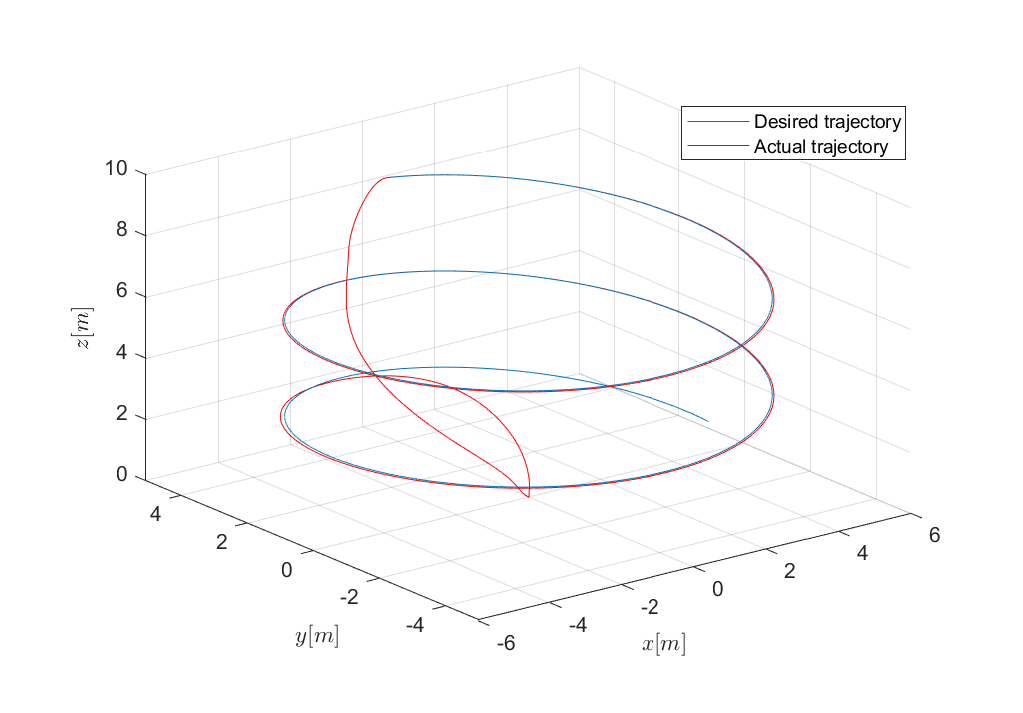
\includegraphics[scale=0.5]{figures/BS_trajectory}
    \caption{Trajectory tracking.}
    \label{fig:BS_trajectory}
\end{figure}
As theoretically expected, the controller exploits the roll and pitch dynamics to impart the desired behavior to the remainder of the system (see Figure \ref{fig:BS_attitude}). 
\begin{figure}[H]
    \centering
    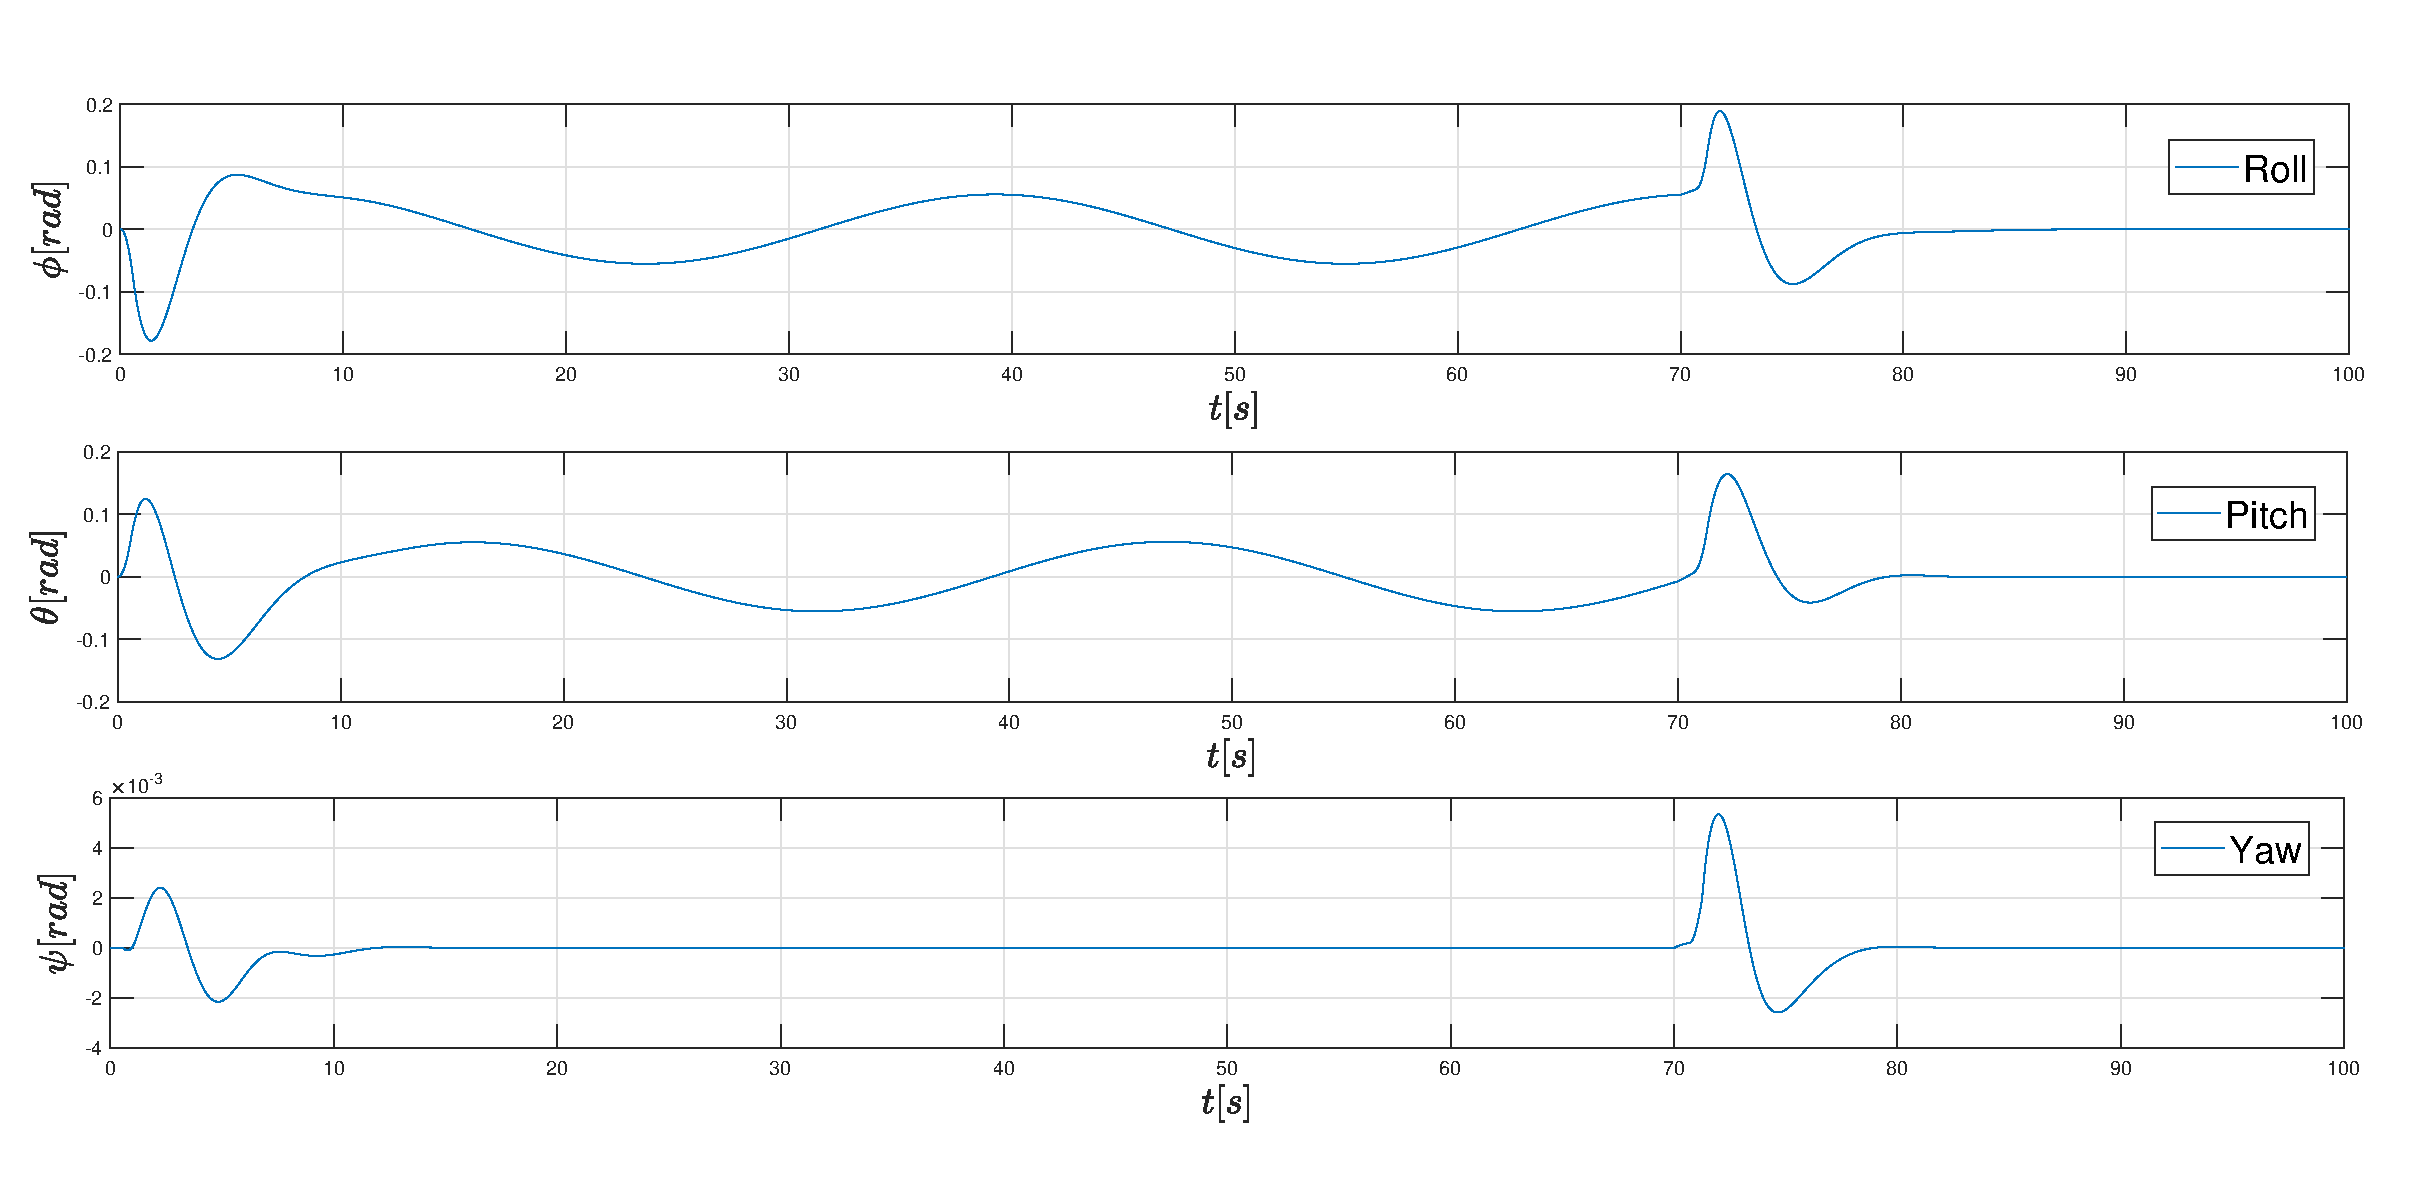
\includegraphics[scale=0.2]{figures/BS_attitude}
    \caption{Evolution of the roll, pitch and yaw angles respectively.}
    \label{fig:BS_attitude}
\end{figure}
Finally, the necessary control inputs, adequately saturated according to the constraints \ref{eq:omega_u_constraint} - \ref{eq:beta_constraint} so as to reflect the actual physical limitations of the actuators, are depicted in Figures \ref{fig:BS_angles} and \ref{fig:BS_omega}. 
\\ We can therefore state that the controller is not only robust to external disturbances, but also to these types of constraints.
\begin{figure}[H]
    \centering
    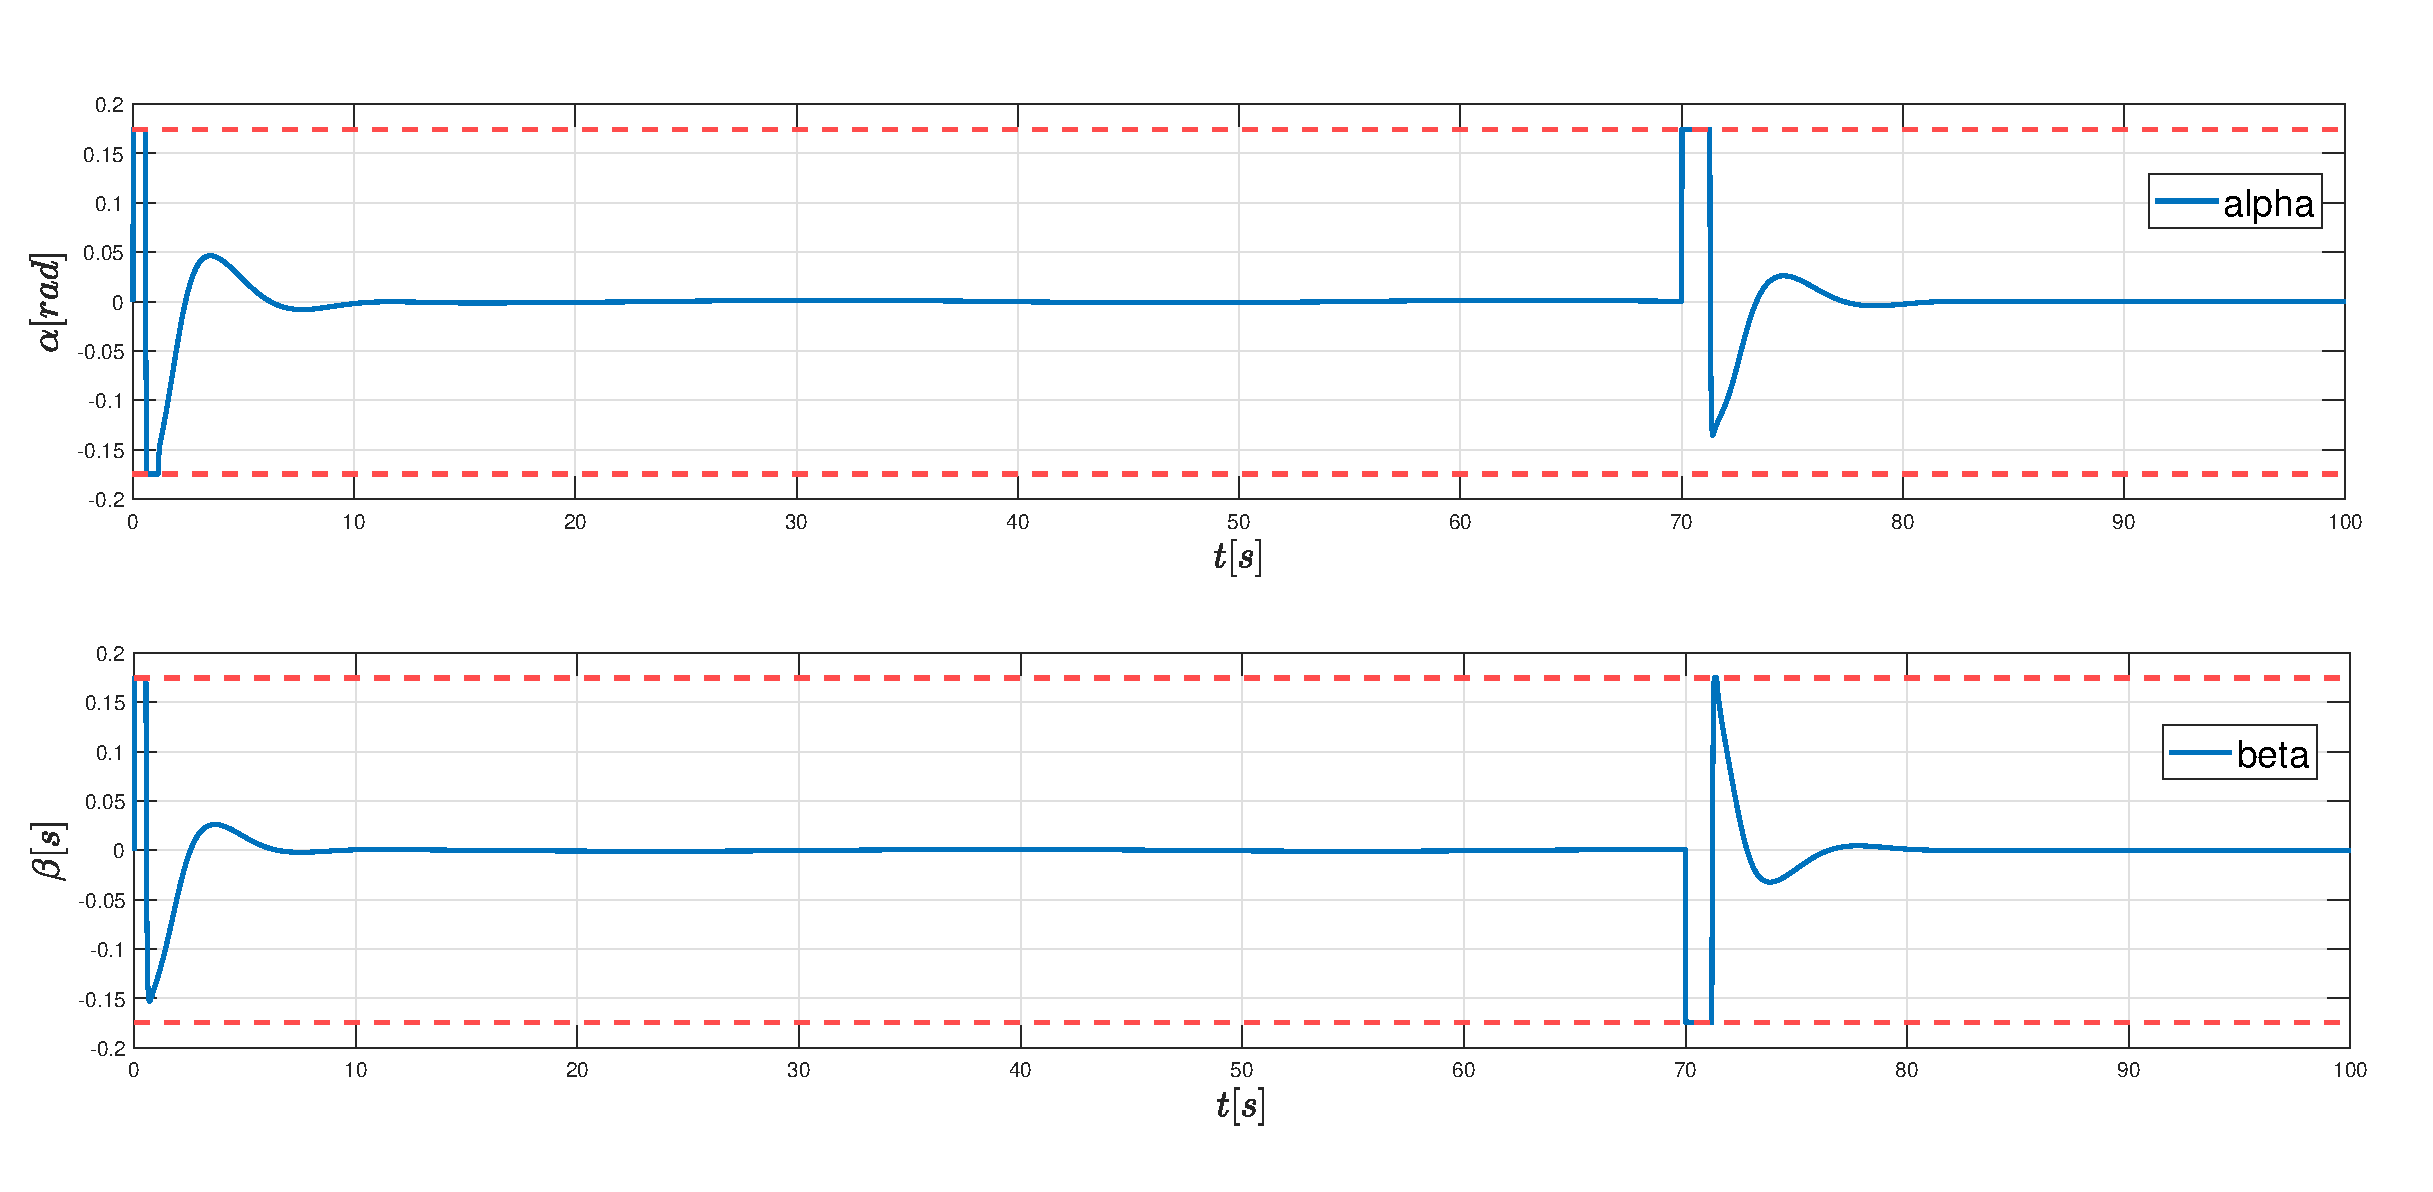
\includegraphics[scale=0.2]{figures/BS_angles}
    \caption{Angles $\alpha$ and $\beta$ of the swashplate.}
    \label{fig:BS_angles}
\end{figure}
\begin{figure}[H]
    \centering
    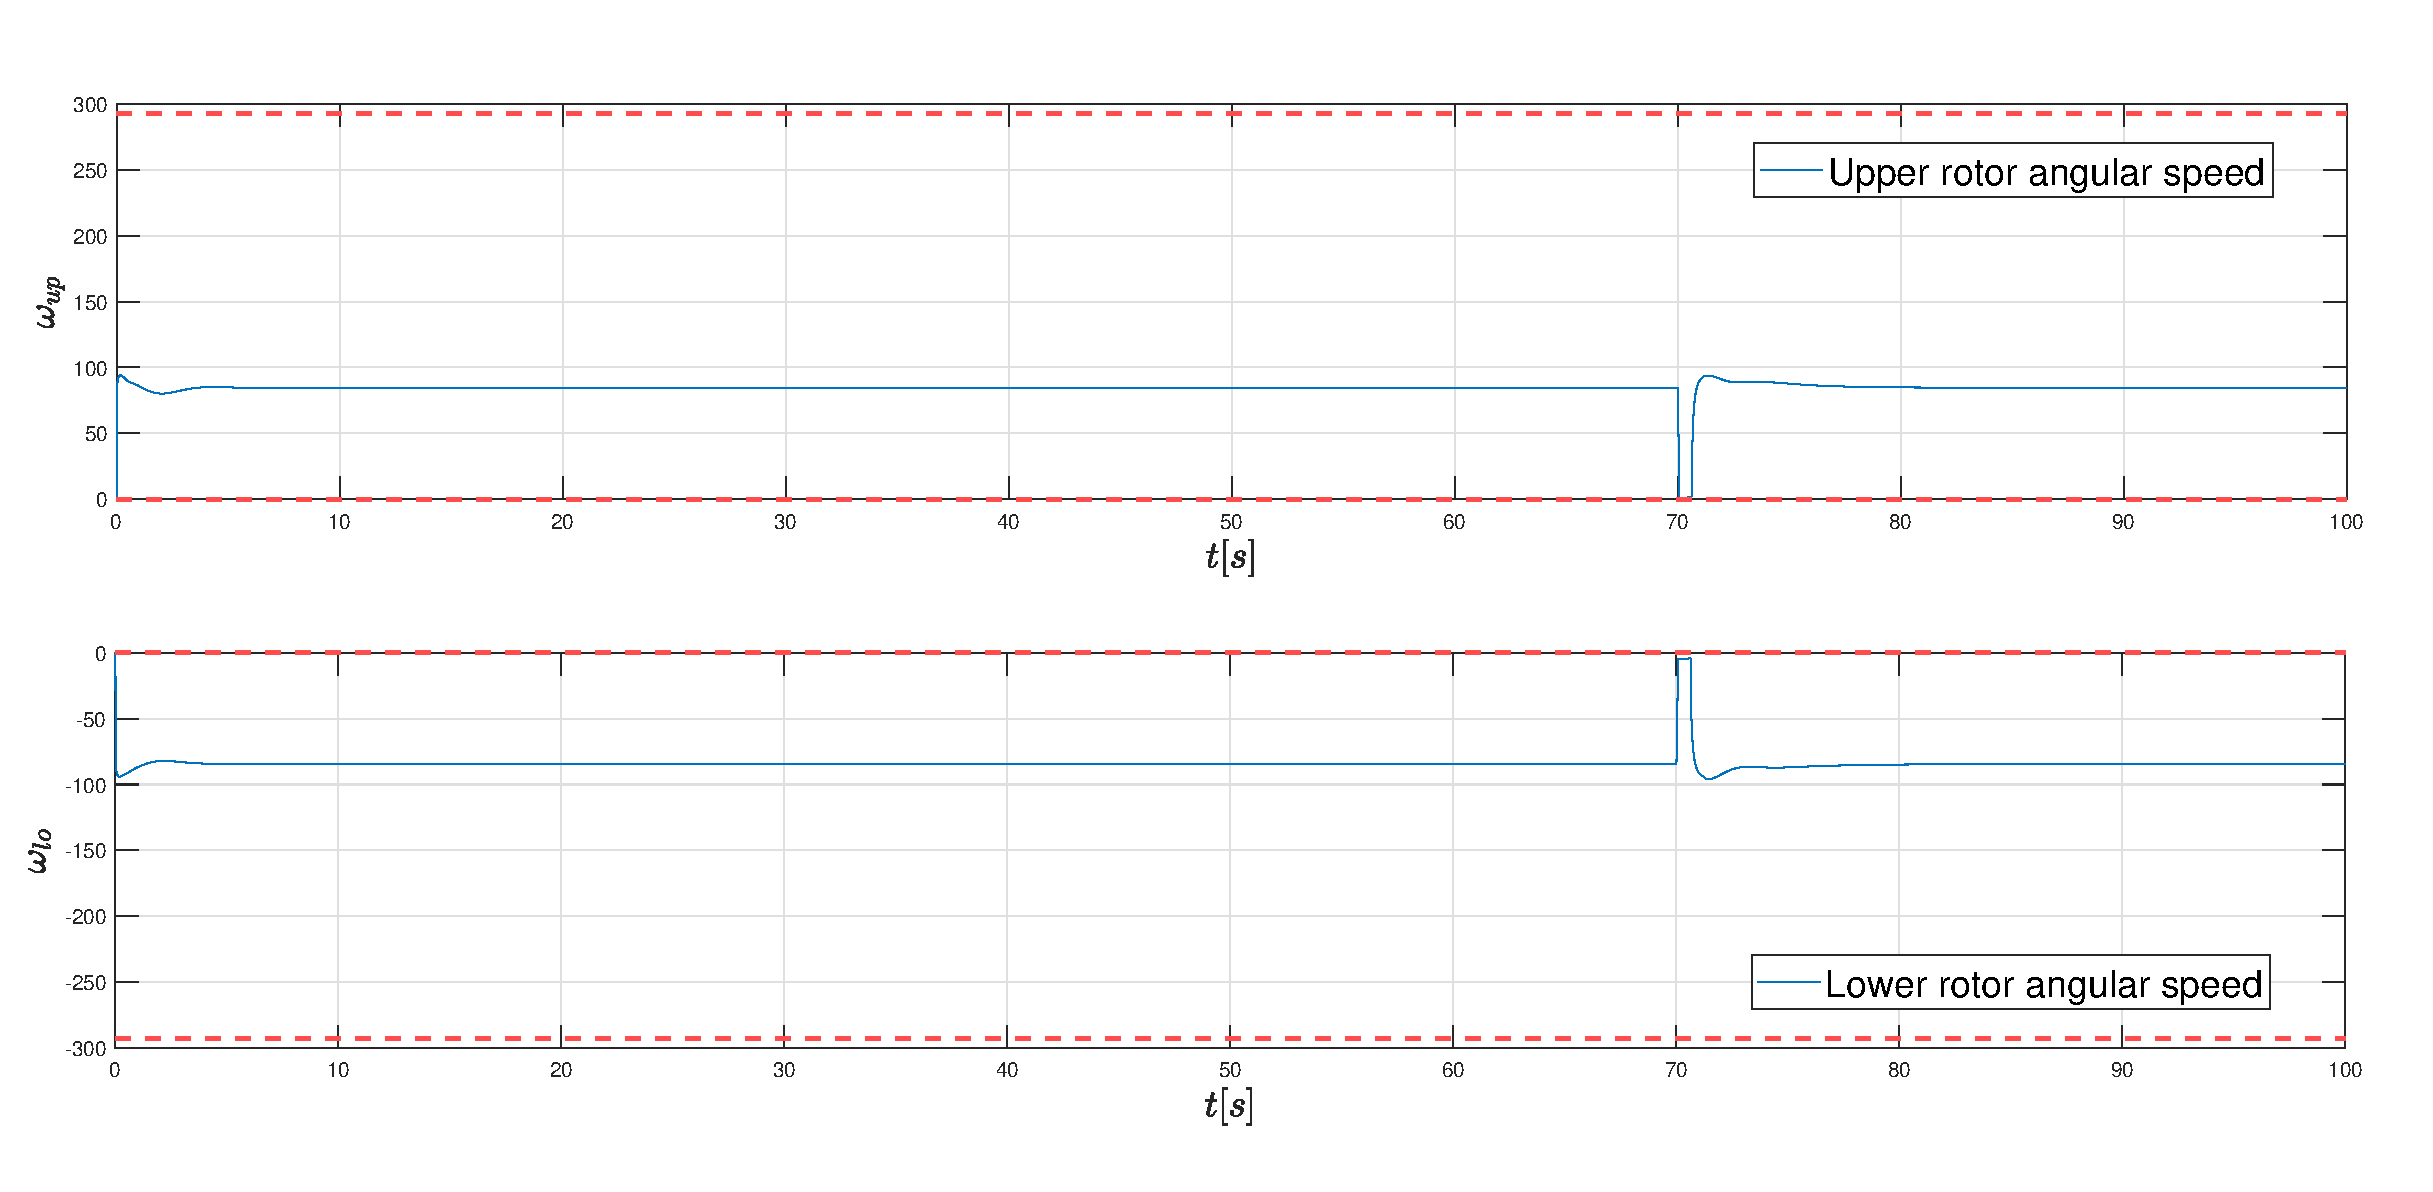
\includegraphics[scale=0.2]{figures/BS_omega}
    \caption{Angular velocities of the upper and lower rotor respectively.}
    \label{fig:BS_omega}
\end{figure}




% \[\frac{d}{dt}L=-(\delta_1+\lambda\delta_2)^T(\delta_1+\lambda\delta_2)-\lambda\delta_2^T\delta_2+(\delta_1+\lambda\delta_2)^T\delta_3+\]\[-K_1\delta_3^T\delta_3-\delta_3^T(\delta_1+\lambda\delta_2)+\delta_3^T\delta_4-K_2\epsilon_2^2+\epsilon_2\epsilon_3-K_4\epsilon_3^2-\epsilon_2\epsilon_3+\]\[-\delta_4^T\delta_3-K_3\delta_4^T\delta_4=
% -(\delta_1+\lambda\delta_2)^T(\delta_1+\lambda\delta_2)-\lambda\delta_2^T\delta_2-K_1\delta_3^T\delta_3+\]\[-K_2\epsilon_2^2-K_4\epsilon_3^2-K_3\delta_4^T\delta_4\]

% The time derivative is 
% \[
% \frac{d}{dt}V_1=(\delta_1+\lambda \delta_2)^T 
% \Bigg[-\Omega^b \times\delta_1+\delta_2+ \lambda\Bigg(-\Omega^b \times\delta_2+\]\[+R^T\ddot{P^d}-\frac{F}{m}\Bigg)\Bigg]+\delta_1^T\left(-\Omega \times \delta_1 +\delta_2\right)=\]\[=(\delta_1+\lambda \delta_2)^T\left(\delta_2+\lambda R^T\ddot{P^d}-\frac{\lambda F}{m}\right)+\delta_1^T\delta_2 \]
% The desired value of the actual force, considered as virtual input gives
% \[\left(\frac{\lambda}{m}F\right)^*=\delta_1+\lambda \delta_2+2\delta_2+\lambda R^T\ddot{P^d}\]
% From which we get 
% \[\frac{d}{dt}V_1=-(\delta_1+\lambda \delta_2)^T(\delta_1+\lambda \delta_2)-\lambda\delta_2^T\delta_2+\]\[+(\delta_1+\lambda \delta_2)^T\frac{\lambda}{m}(F^*-F)\]
% where the error between the virtual force
% and the actual force $\delta_3=(\frac{\lambda}{m}F)^*-\frac{\lambda}{m}F $ appears.\\
% Its derivative is 
% \[\frac{d}{dt}\delta_3=\frac{d}{dt}\left(\frac{\lambda}{m}F\right)^*-\frac{d}{dt}\left(\frac{\lambda}{m}F\right)=\]\[=
% \frac{d}{dt}(\delta_1+\lambda \delta_2+2\delta_2+\lambda R^T\ddot{P^d})-\frac{\lambda}{m}\frac{d}{dt}(R^TF_g^i+u)=\]\[=
% -\Omega^b \times \delta_1+\delta_2+(\lambda+2)\left(-\Omega^b \times \delta_2+R^T\ddot{P^d}-\frac{F}{m}\right)+\]\[+\lambda R^T\dddot{P^d}-\lambda\Omega^b \times R^T\ddot{P^d}+\frac{\lambda}{m}\Omega^b \times R^TF_g^i-\frac{\lambda}{m}\left(\frac{d}{dt}u\right)=\]\[=
% -\Omega^b \times \left(\delta_1+\lambda \delta_2+2\delta_2+\lambda R^T\ddot{P^d}-\frac{\lambda}{m} R^TF_g^i-\frac{\lambda}{m}u\right)\]\[-\frac{\lambda}{m}\Omega^b \times u+\delta_2+(\lambda+2)\left(R^T\ddot{P^d}-\frac{F}{m}\right)+\]\[+\lambda R^T\dddot{P^d}-\frac{\lambda}{m}\left(\frac{d}{dt}u\right)=
% -\Omega^b \times \delta_3 -\frac{\lambda}{m}\Omega^b \times u+\]\[+\frac{\lambda+2}{\lambda}\left(\lambda R^T\ddot{P^d}-\frac{\lambda}{m}F+\delta_1+\lambda \delta_2+2\lambda_2\right)+\]\[-\frac{\lambda+2}{\lambda}\left(\delta_1+\lambda \delta_2+2\lambda_2\right)+\delta_2+\lambda R^T\dddot{P^d}-\frac{\lambda}{m}\left(\frac{d}{dt}u\right)=\]\[=
% -\Omega^b \times \delta_3 -\frac{\lambda}{m}\Omega^b \times u+\frac{\lambda+2}{\lambda}\delta_3-\frac{\lambda+2}{\lambda}\delta_1-\frac{(\lambda+2)^2-\lambda}{\lambda}\delta_2+\]\[+\lambda R^T\dddot{P^d}-\frac{\lambda}{m}\left(\frac{d}{dt}u\right)
% \]
% Regarding the yaw control, we have the error
% \[\epsilon_2 := w_{3,d}-w_3\]
% and its derivative
% \[\frac{d}{dt}\epsilon_2=\dot{w_{3,d}}-\frac{d}{dt}w_3\]
% The second Lyapunov function is then
% \[V_2=\frac{1}{2}\delta_3^T\delta_3+\frac{1}{2}\epsilon_2^2\]
% Differentiating we get
% \[\frac{d}{dt}V_2=\delta_3^T\Bigg[-\Omega^b \times \delta_3-\frac{\lambda}{m}\Omega^b \times u+\frac{\lambda+2}{\lambda}\delta_3-\frac{\lambda+2}{\lambda}\delta_1+\]\[-\frac{(\lambda+2)^2-\lambda}{\lambda}\delta_2+\lambda R^T\dddot{P^d}-\frac{\lambda}{m}\left(\frac{d}{dt}u\right)\Bigg]+\epsilon_2\left(\dot{w_{3,d}}-\frac{d}{dt}w_3\right)\]
% Since $\frac{d}{dt}u$ and $\Omega$ are completely decoupled we can affect directly the input $\frac{d}{dt}u$. In particular we impose
% \[\frac{d}{dt}u_3=\frac{m}{\lambda}\begin{bmatrix}
% 0 & 0 &1 \end{bmatrix}\Bigg(\frac{\lambda+2}{\lambda}\delta_3-\frac{\lambda+2}{\lambda}\delta_1-\frac{\lambda^2+3\lambda+4}{\lambda}\delta_2+\]\[+\lambda R^T\dddot{P^d}+(\delta_1+\lambda\delta_2)+K_1\delta_3\Bigg)\]
% While we choose the control inputs
% \[\left(\frac{\lambda}{m}\Omega^b \times u\right)^*=
% \begin{bmatrix}
%     1 & 0 & 0 \\ 0 & 1 & 0 \\ 0 & 0 & 0
% \end{bmatrix}\Bigg(\frac{\lambda+2}{\lambda}\delta_3-\frac{\lambda+2}{\lambda}\delta_1+\]\[-\frac{\lambda^2+3\lambda+4}{\lambda}\delta_2+\lambda R^T\dddot{P^d}+(\delta_1+\lambda\delta_2)+K_1\delta_3\Bigg)\]
% \[\left(\frac{d}{dt}w_3\right)^*=\frac{d}{dt}w_3+K_2\epsilon_2 \:\:, \quad K_1,K_2>0\]

% The derivative of $V_2$ becomes
% \[\frac{d}{dt}V_2=-K_1\delta_3^T\delta_3-\delta_3^T(\delta_1+\lambda\delta_2)+\delta_3^T\Bigg[\Bigg(\frac{\lambda}{m}\Omega^b \times u\Bigg)^*+\]\[-\frac{\lambda}{m}\Omega^b \times u\Bigg]-K_2\epsilon_2^2+\epsilon_2\left(\left(\frac{d}{dt}w_3\right)^*-\dot{w_3}\right)\]
% \\
% The new vector error associated with
% the speed rotations in roll and pitch is 
% \[\delta_4:=\left(\frac{\lambda}{m}\Omega^b \times u\right)^*-\frac{\lambda}{m}\Omega^b \times u\]
% Its derivative is
% \[\frac{d}{dt}\delta_4=\frac{d}{dt}\left(\frac{\lambda}{m}\Omega^b \times u\right)^*-\frac{\lambda}{m}\left(\frac{d}{dt}\Omega^b\right)\times u+\]\[-\frac{\lambda}{m}\Omega^b \times \left(\frac{d}{dt}u\right)\]
% \\
% The yaw speed error is instead 
% \[\epsilon_3:=\dot{w_3}^*-\frac{d}{dt}w_3\]
% and its derivative
% \[\frac{d}{dt}\epsilon_3=\frac{d}{dt}(\dot{w_{3,d}}+K_2\epsilon_2)-\frac{d^2}{dt^2}w_3=\]\[=\ddot{w_{3,d}}+K_2\left(\dot{w_{3,d}}-\frac{d}{dt}w_3\right)-\frac{d^2}{dt^2}w_3\]
% The last Lyapunov function is given by
% \[V_3=\frac{1}{2}\delta_4^T\delta_4+\frac{1}{2}\epsilon_3^2\]
% Taking the time derivative it yields
% \[\frac{d}{dt}V_3=\delta_4^T\Bigg[\frac{d}{dt}\Bigg(\frac{\lambda}{m}\Omega^b \times u\Bigg)^*+\]\[-\frac{\lambda}{m}\Bigg(\frac{d}{dt}\Omega^b\Bigg) \times u-\frac{\lambda}{m}\Omega^b \times \Bigg(\frac{d}{dt}u\Bigg) \Bigg]+\]\[+\epsilon_3\left[\ddot{w_{3,d}}+K_2\left(\dot{w_{3,d}}-\frac{d}{dt}w_3\right)-\frac{d^2}{dt^2}w_3\right]\]

% At this point we choose
% \[\frac{d^2}{dt^2}w_3= \ddot{w_{3,d}}+K_2\Bigg(\dot{w_{3,d}}-\frac{d}{dt}w_3\Bigg)+K_4\epsilon_3+\epsilon_2\]
% \\
% \[\frac{\lambda}{m}\left(\frac{d}{dt}\Omega^b\right) \times u=\frac{d}{dt}\left(\frac{\lambda}{m}\right)^*-\frac{\lambda}{m}\Omega^b\times\left(\frac{d}{dt}u\right)+\]\[+\begin{bmatrix}
%     1 & 0 & 0 \\ 0 & 1 & 0 \\ 0 & 0 & 0 
% \end{bmatrix}\delta_3+K_3\delta_4\]

% In particular from the latter we would have
% \[\frac{\lambda}{m}\begin{bmatrix}
%     \left(\frac{d}{dt}\Omega_2^b\right)u_3 \\ -\left(\frac{d}{dt}\Omega_1^b\right)u_3
% \end{bmatrix}=\begin{bmatrix}
%     1 & 0 & 0 \\ 0 & 1 & 0
% \end{bmatrix}\Bigg[\frac{d}{dt}\Bigg(\frac{\lambda}{m}\Omega^b\times u\Bigg)^*+\]\[-\frac{\lambda}{m}\Omega^b\times \dot u +\delta_3+K_3\delta_4\Bigg]\]
% and so in the end
% \[\frac{d}{dt}\Omega_2^b=\frac{m}{\lambda u_3}\begin{bmatrix}
%     1 & 0 & 0
% \end{bmatrix}\Bigg[\frac{d}{dt}\left(\frac{\lambda}{m}\Omega^b\times u\right)^*-\frac{\lambda}{m}\Omega^b \times \dot u +\delta_3+K_3\delta_4\Bigg]\]

% \[\frac{d}{dt}\Omega_1^b=-\frac{m}{\lambda u_3}\begin{bmatrix}
%     0 & 1 & 0
% \end{bmatrix}\Bigg[\frac{d}{dt}\left(\frac{\lambda}{m}\Omega^b\times u\right)^*-\frac{\lambda}{m}\Omega^b \times \dot u +\delta_3+K_3\delta_4\Bigg]\]

% In this way the derivative of the third Lyapunov function becomes
% \[\frac{d}{dt}V_3=-K_4\epsilon_3^2-\epsilon_2\epsilon_3-\delta_4^T\delta_3-K_3\delta_4^T\delta_4\]
% \\
% Summing up the three Lyapunov functions we get
% \[L=V_1+V_2+V_3=\frac{1}{2}(\delta_1+\lambda\delta_2)^T(\delta_1+\lambda\delta_2)+\]\[+\frac{1}{2}\delta_1^T\delta_1+\frac{1}{2}\delta_3^T\delta_3+\frac{1}{2}\epsilon_2^2+\frac{1}{2}\delta_4^T\delta_4+\frac{1}{2}\epsilon_3^2\]
% Whose derivative is 
% \[\frac{d}{dt}L=-(\delta_1+\lambda\delta_2)^T(\delta_1+\lambda\delta_2)-\lambda\delta_2^T\delta_2+(\delta_1+\lambda\delta_2)^T\delta_3+\]\[-K_1\delta_3^T\delta_3-\delta_3^T(\delta_1+\lambda\delta_2)+\delta_3^T\delta_4-K_2\epsilon_2^2+\epsilon_2\epsilon_3-K_4\epsilon_3^2-\epsilon_2\epsilon_3+\]\[-\delta_4^T\delta_3-K_3\delta_4^T\delta_4=
% -(\delta_1+\lambda\delta_2)^T(\delta_1+\lambda\delta_2)-\lambda\delta_2^T\delta_2-K_1\delta_3^T\delta_3+\]\[-K_2\epsilon_2^2-K_4\epsilon_3^2-K_3\delta_4^T\delta_4\]

% We can see that the overall Lyapunov function is monotonically decreasing and thus the control objective is achieved.
